\documentclass[12pt, a4paper]{article}

\usepackage[a4paper, margin=2cm]{geometry}
\usepackage{setspace}
\usepackage[portuguese]{babel}
\usepackage{graphicx}
\usepackage{hyperref}
\usepackage{amsfonts}
\usepackage[dvipsnames]{xcolor}

\chardef\_=`_

\title{\textbf{LI3 - Relatório da Fase II - Grupo 12}}
\author{
    Humberto Gomes (A104348) \\
    José Lopes     (A104541) \\
    José Matos     (A100612) \\
}
\date{janeiro de 2024}

\begin{document}
\maketitle
\onehalfspacing
\setlength{\parskip}{\baselineskip}
\setlength{\parindent}{0pt}

\begin{abstract}
    Após a conclusão da primeira fase deste trabalho, procurámos implementar as funcionalidades em
    falta para a conclusão do desenvolvimento desta aplicação: as restantes quatro
    \emph{queries}, um modo de uso interativo (uma interface TUI), testes funcionais e de
    desempenho, e suporte para um \emph{dataset} de maior dimensão, mantendo um desempenho
    aceitável. Adicionalmente, procurámos também melhorar o encapsulamento e a modularidade no
    nosso projeto.
\end{abstract}

\section{Estrutura do trabalho}

Nesta secção, procuramos descrever as diferenças entre a nossa arquitetura modular atual, e a que
tínhamos presente na primeira fase do projeto. Devido ao elevado número de módulos, após o diagrama
de dependências completo que se segue, este documento descreve o funcionamento de cada subsistema
lógico do programa um a um. Nestes esquemas, para reduzir a complexidade visual, não incluímos
todas as relações de dependência, mas apenas as mais relevantes. Segue-se a nossa convenção gráfica:

\begin{itemize}
    \item Um retângulo com cantos arredondados representa uma estrutura de dados;
    \item Um retângulo sem cantos arredondados representa um módulo cuja tarefa principal é a
          execução de código. No entanto, alguns destes módulos podem conter estruturas de dados
          auxiliares (por exemplo, uma gramática definida no módulo de um \emph{parser});
    \item $A \rightarrow B$ significa que o módulo $A$ depende do módulo $B$.
    \item Qualquer módulo ou relação de dependência representado(a) a {\color{ForestGreen}verde}
          indica que o(a) mesmo(a) é uma adição nesta segunda fase, ausente na entrega anterior.
\end{itemize}

% TODO - inserir diagrama global aqui

\subsection{\emph{Parsing}}
\label{sec:parsing}

\begin{figure}[ht]
    \centering
    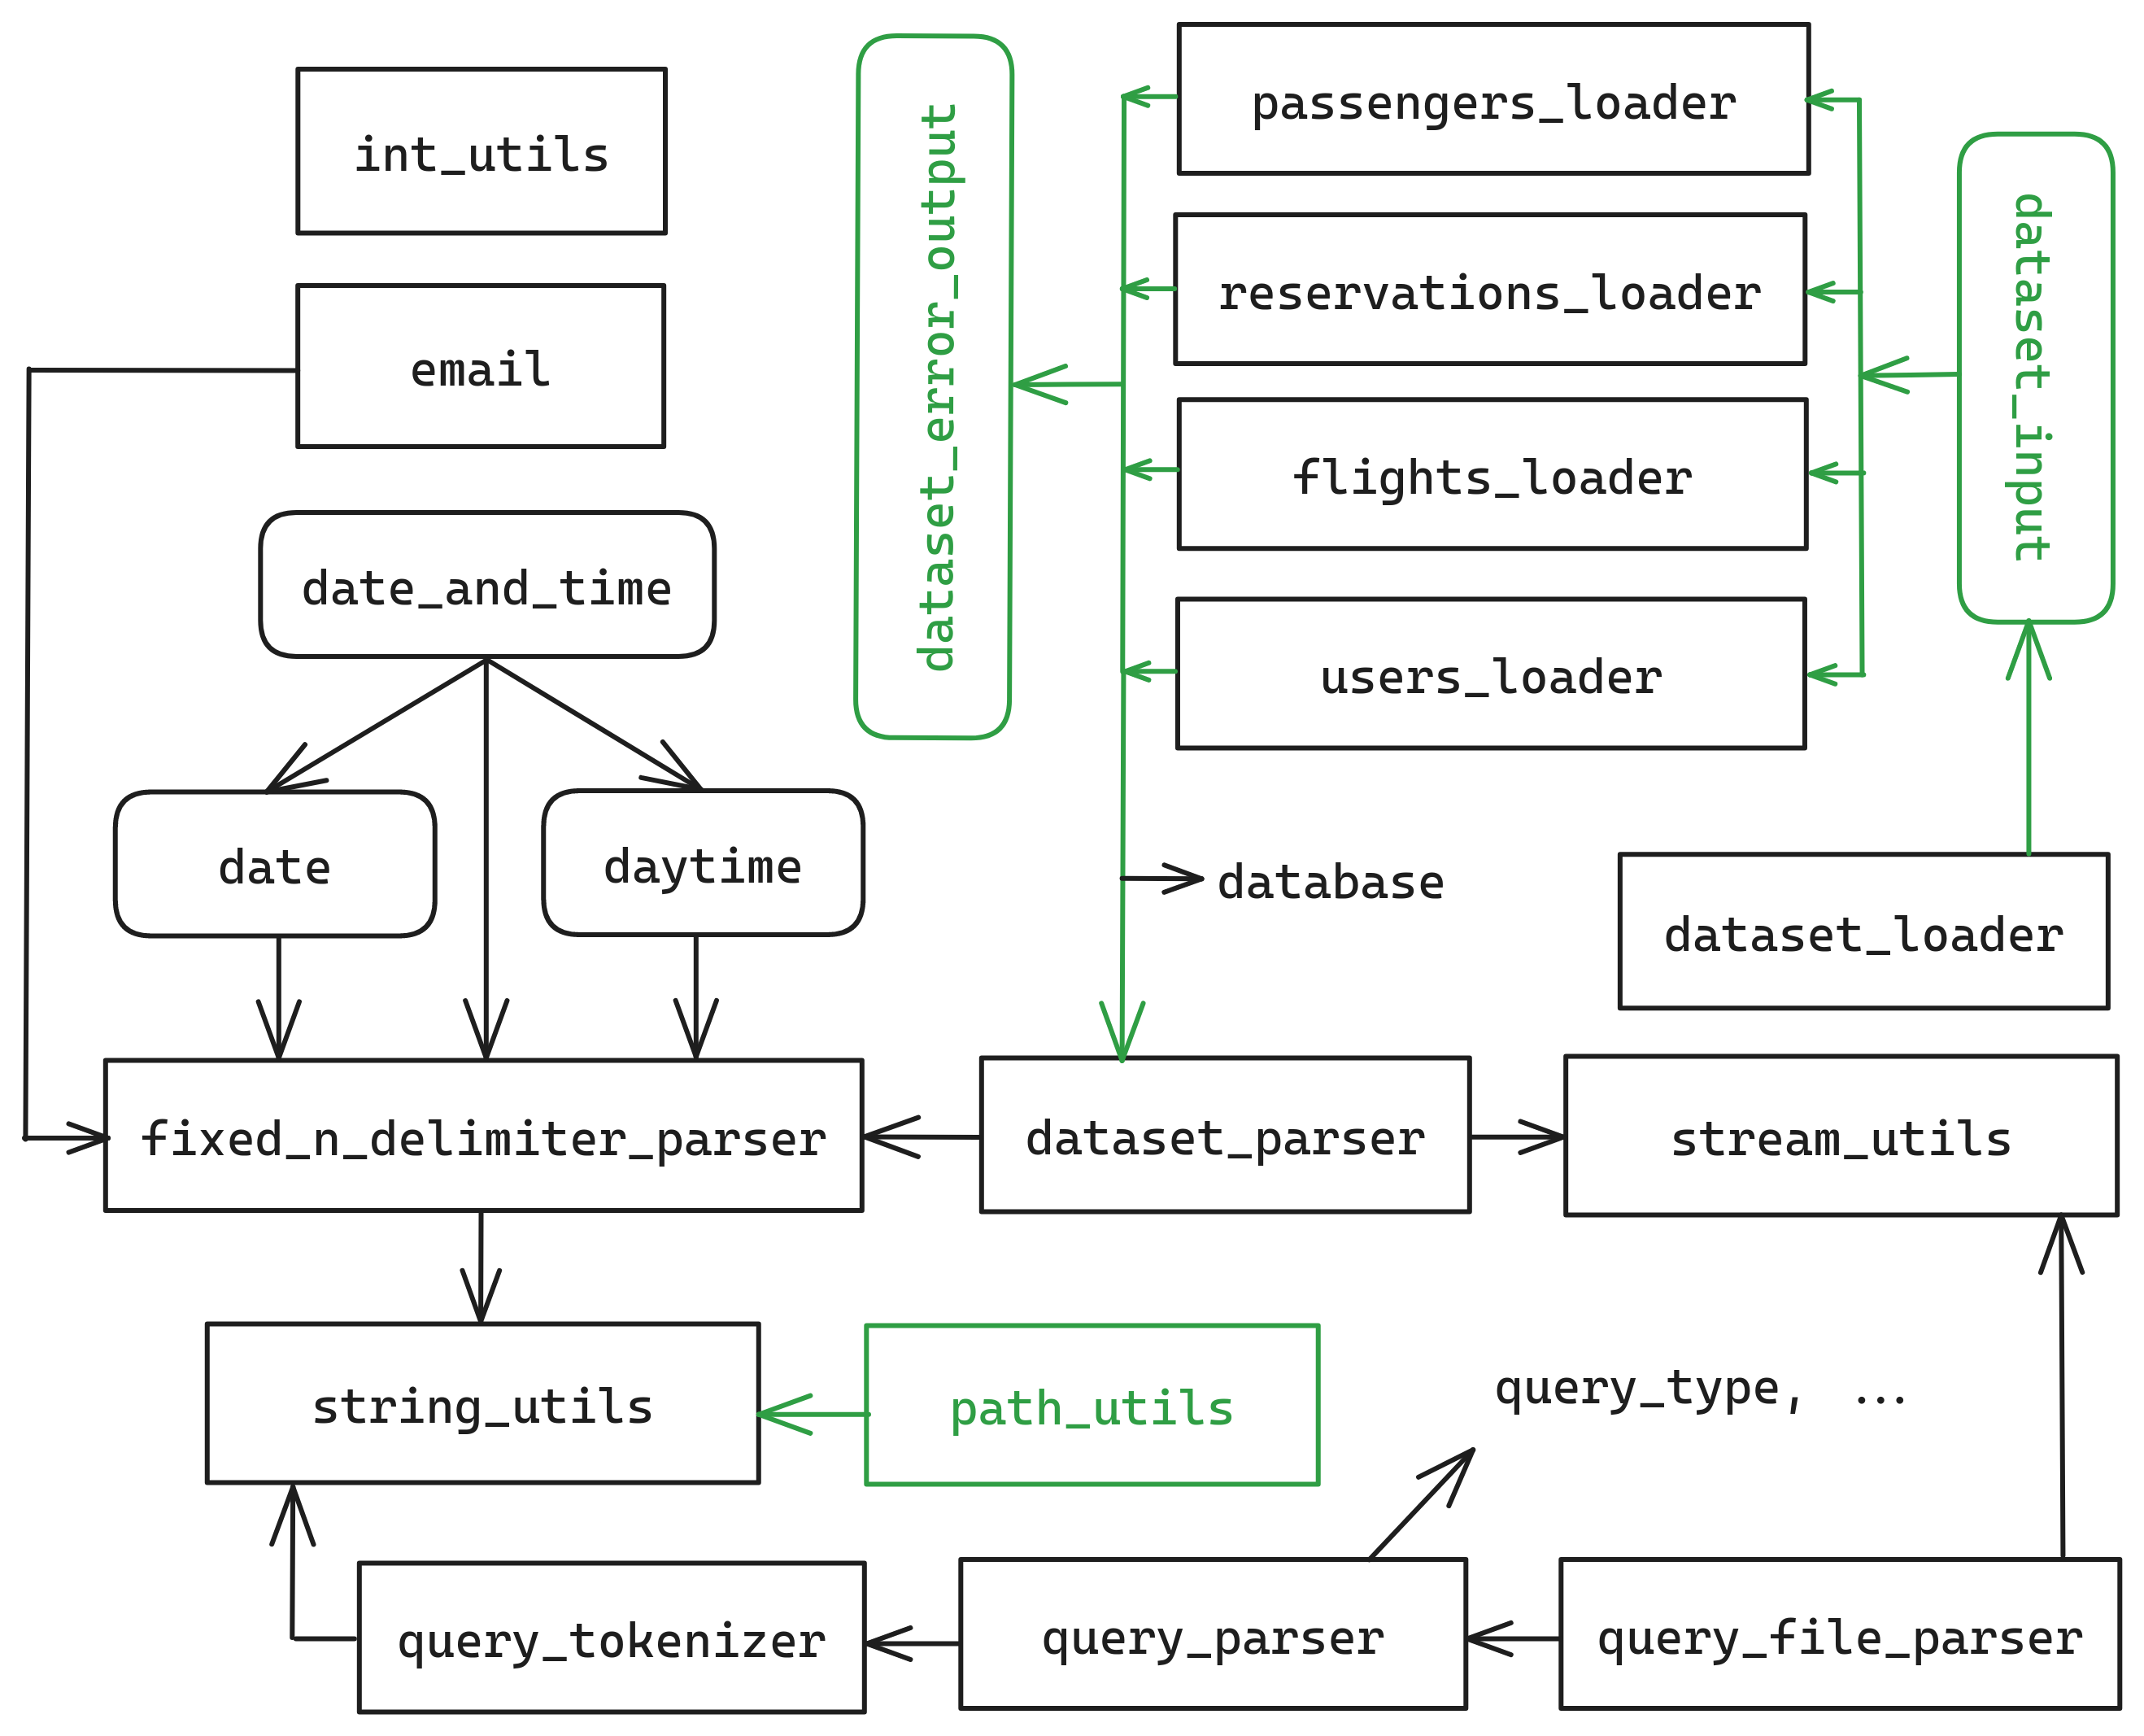
\includegraphics[scale=0.17]{res-fase2/parsing.png}
    \caption{Diagrama de dependências do subsistema de \emph{parsing}}
    \label{fig:parsing}
\end{figure}

Nesta fase do projeto, separámos as funcionalidades de \emph{input} de dados e \emph{output} de
erros num \emph{dataset}, antes concentradas no módulo \texttt{dataset\_loader}. Agora, este módulo
gere duas estruturas de dados distintas, \texttt{dataset\_input} e \texttt{dataset\_error\_output},
formadas por \emph{handles} de ficheiros abertos para leitura / escrita. Ademais, adicionámos o
módulo \texttt{path\_utils}, para manipulação de caminhos para ficheiros.

\subsection{Entidades}
\label{sec:entities}

\begin{figure}[ht]
    \centering
    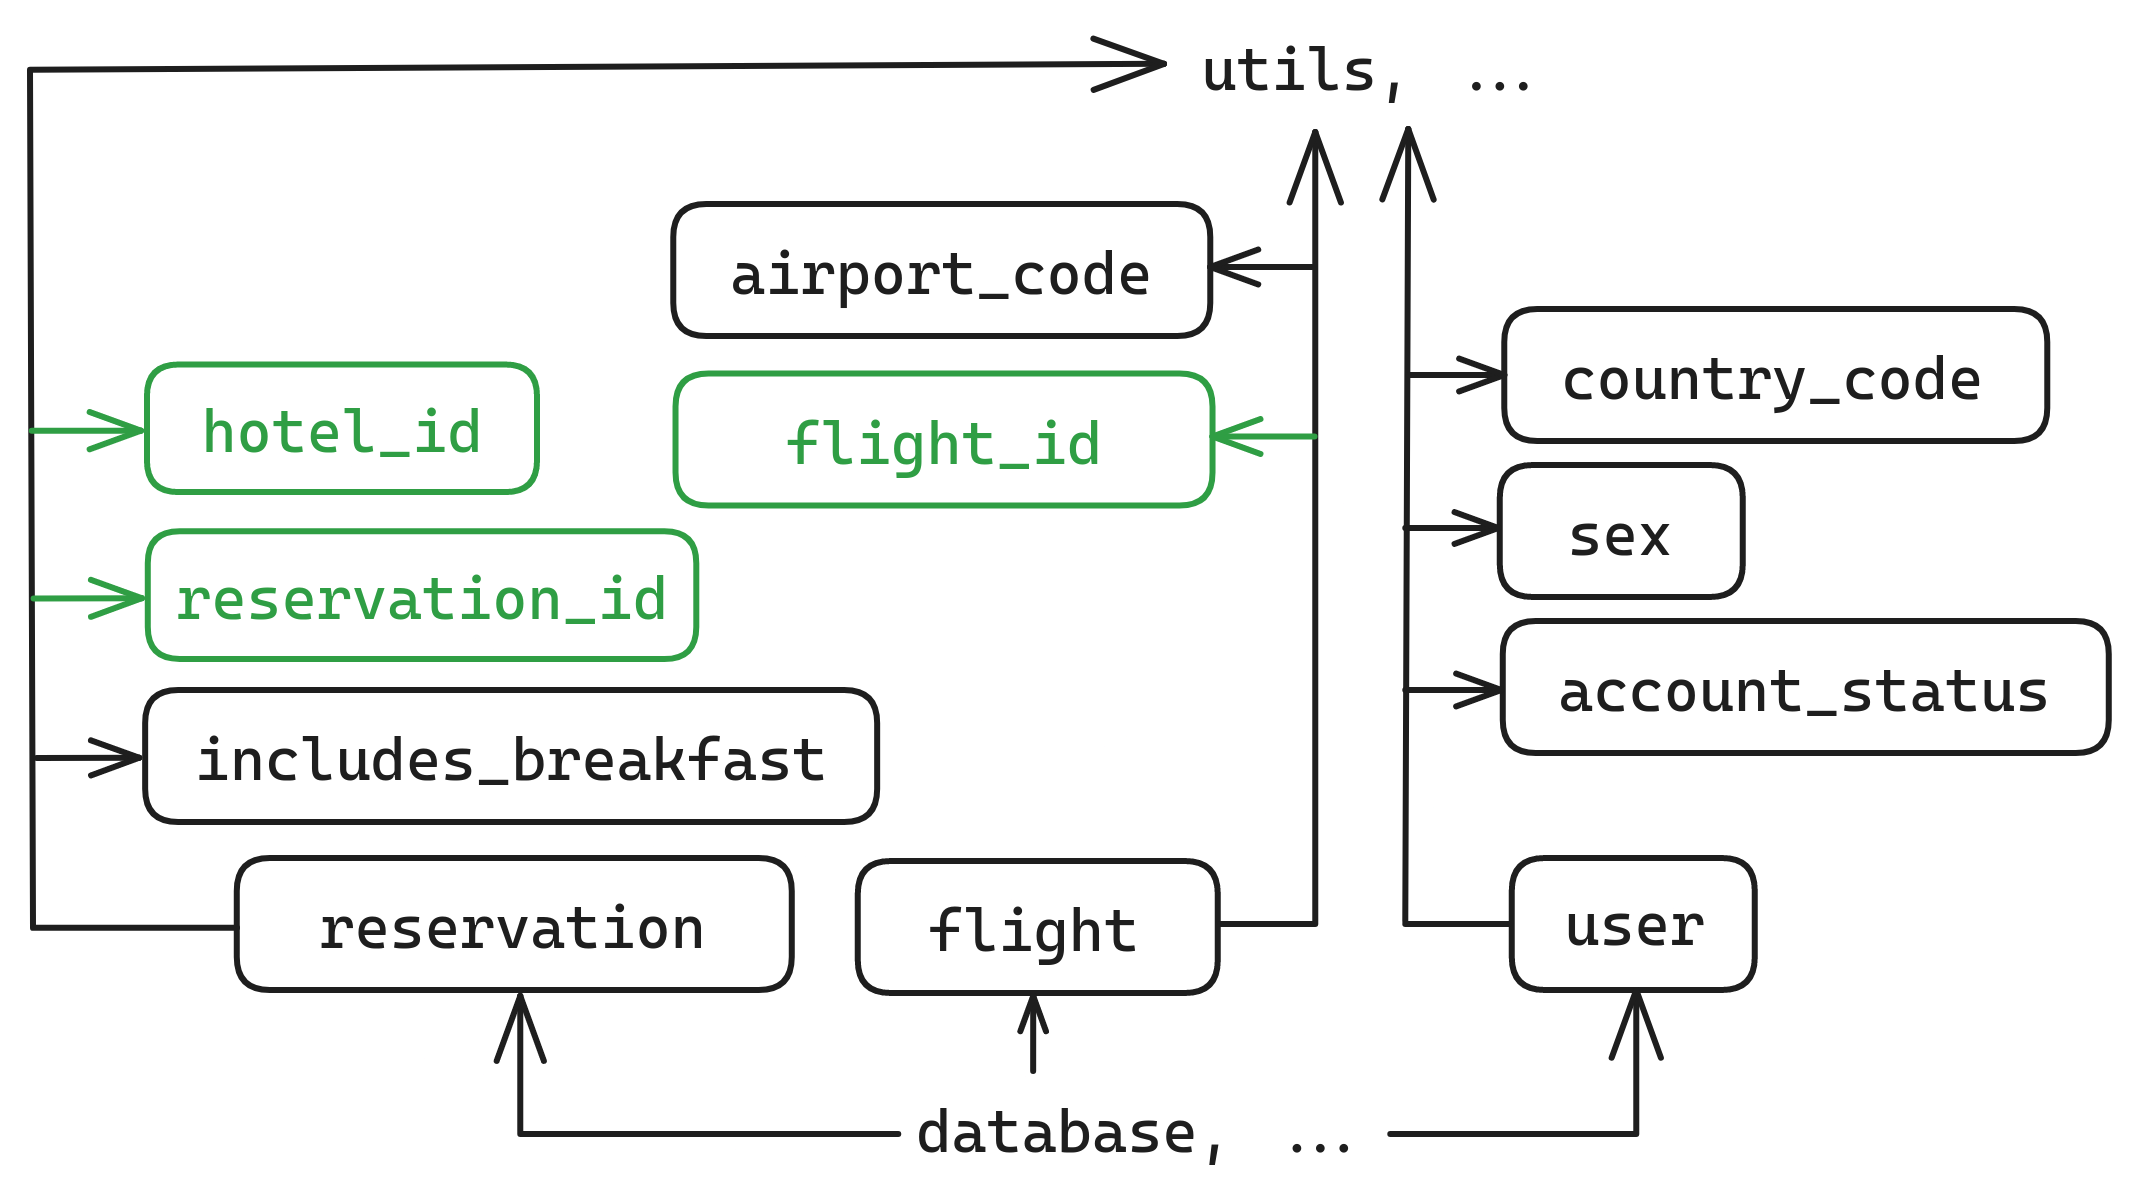
\includegraphics[scale=0.2]{res-fase2/entities.png}
    \caption{Diagrama de dependências das entidades da aplicação}
    \label{fig:entities}
\end{figure}

Nas entidades, criámos módulos para os identificadores de voos, reservas e hotéis. Estes são
armazenados como inteiros, e consequentemente exigem \emph{parsing} e uma forma de serem
apresentados textualmente, código que antes se encontrava em duplicado em vários locais da
aplicação.

\subsection{Catálogos}
\label{sec:catalogs}

\begin{figure}[ht]
    \centering
    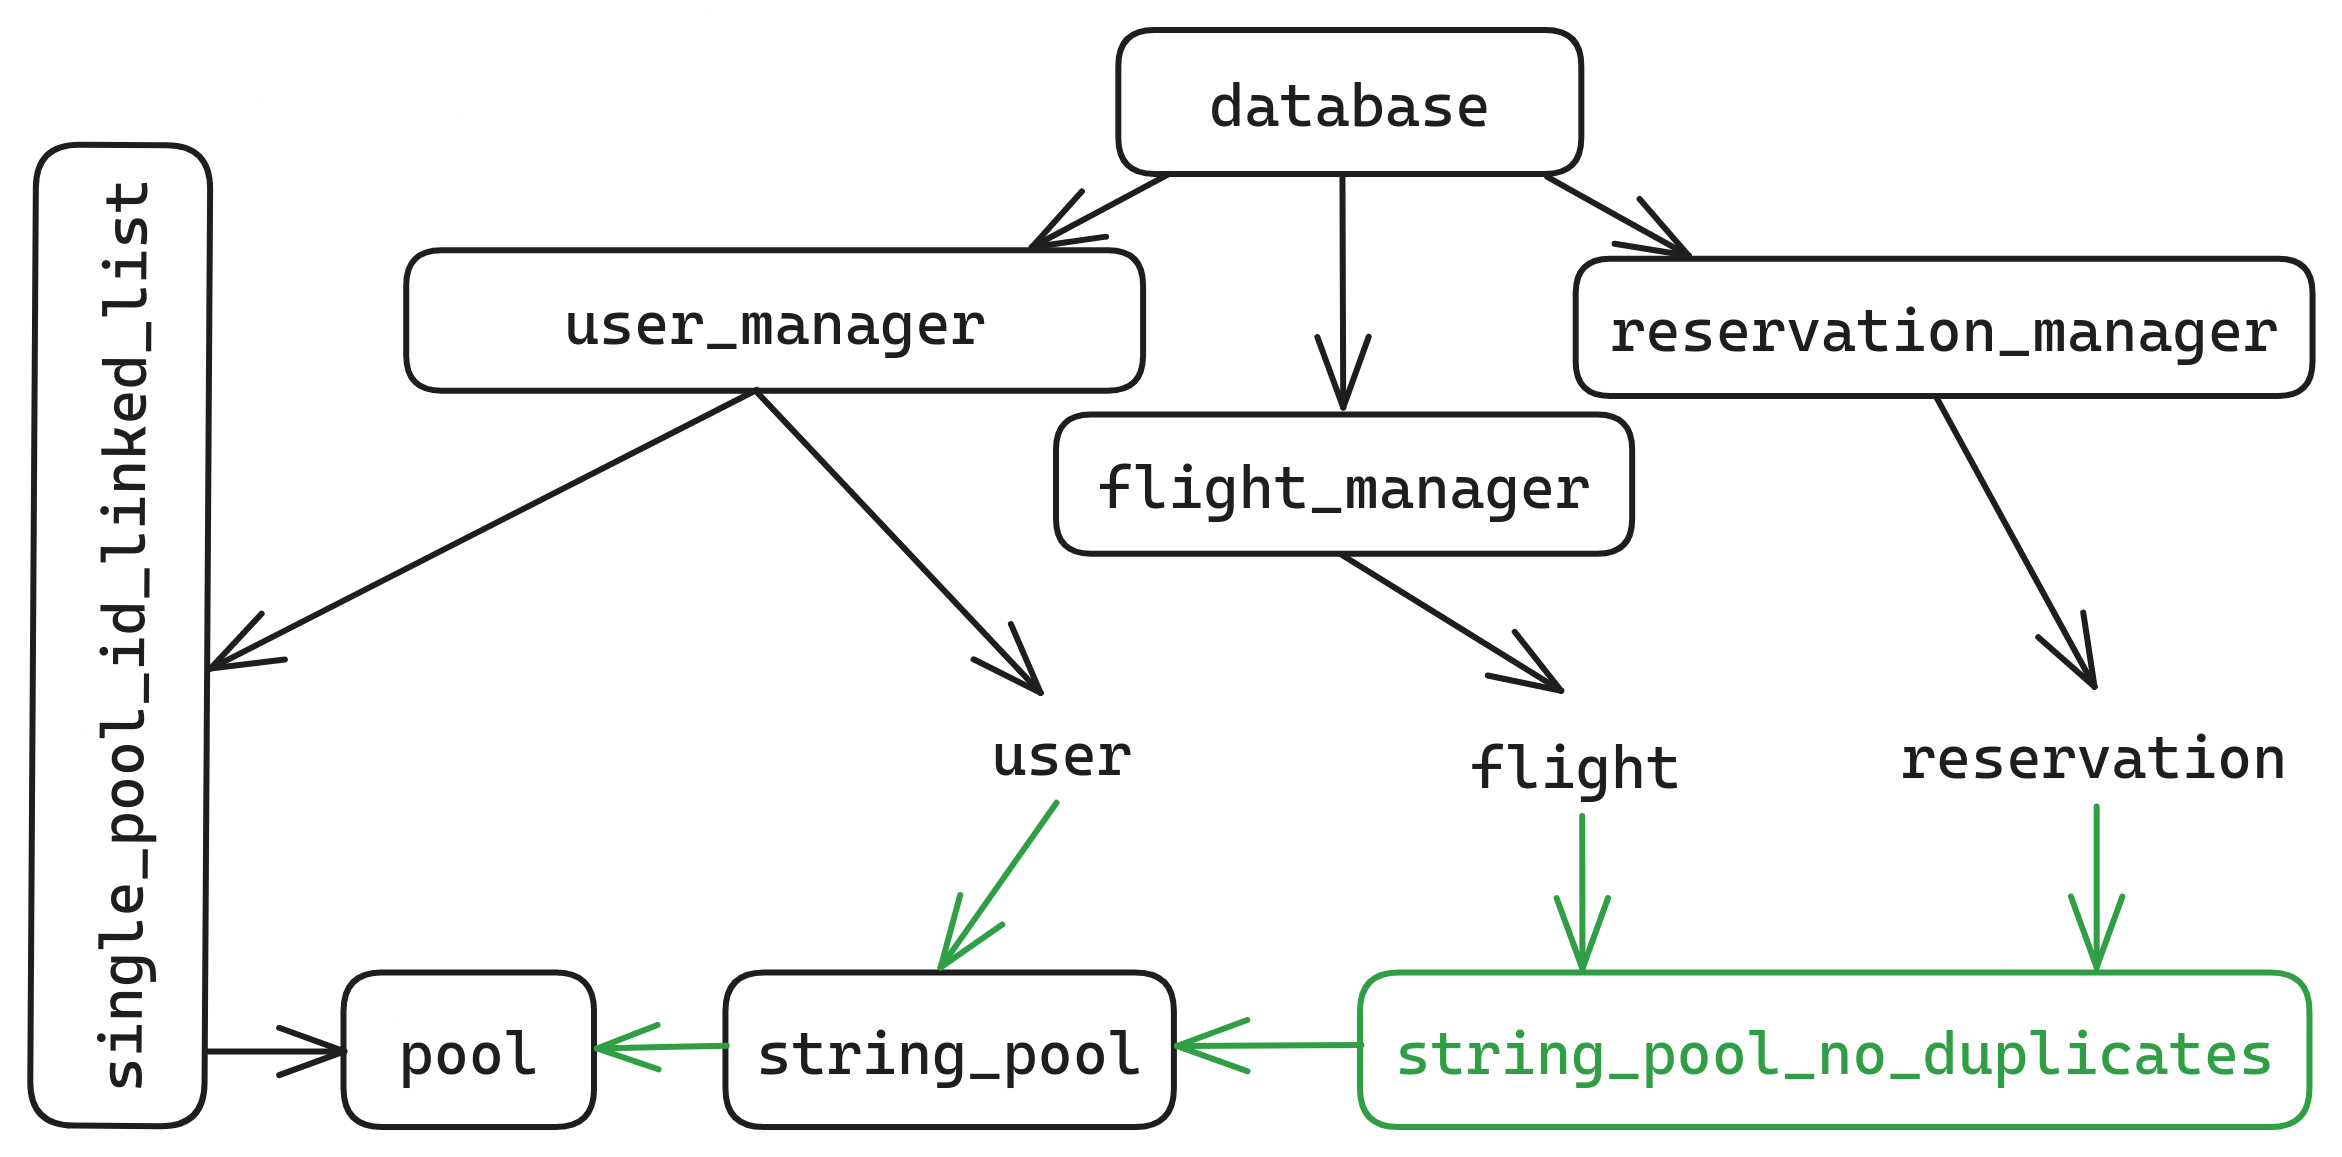
\includegraphics[scale=0.17]{res-fase2/database.png}
    \caption{Diagrama de dependências dos catálogos na aplicação}
    \label{fig:catalogs}
\end{figure}

De modo a diminuir o uso de memória da aplicação ainda mais, procurámos comprimir campos do
\emph{dataset} com baixa entropia, como nomes de hotéis e de companhias aéreas, que surgem várias
vezes repetidos. Para isso, criámos um novo alocador que armazena \emph{strings} repetidas apenas
uma vez, o \texttt{string\_pool\_no\_duplicates}.

Quanto às novas relações de dependência, reimplementámos a \texttt{string\_pool} utilizando uma
\texttt{pool}, para melhor reutilização de código. Ademais, agora as entidades passam a depender
dos alocadores, por motivos explicados em \nameref{sec:modularity-and-encapsulation}.

\subsection{\emph{Queries}}
\label{sec:queries}

\begin{figure}[ht]
    \centering
    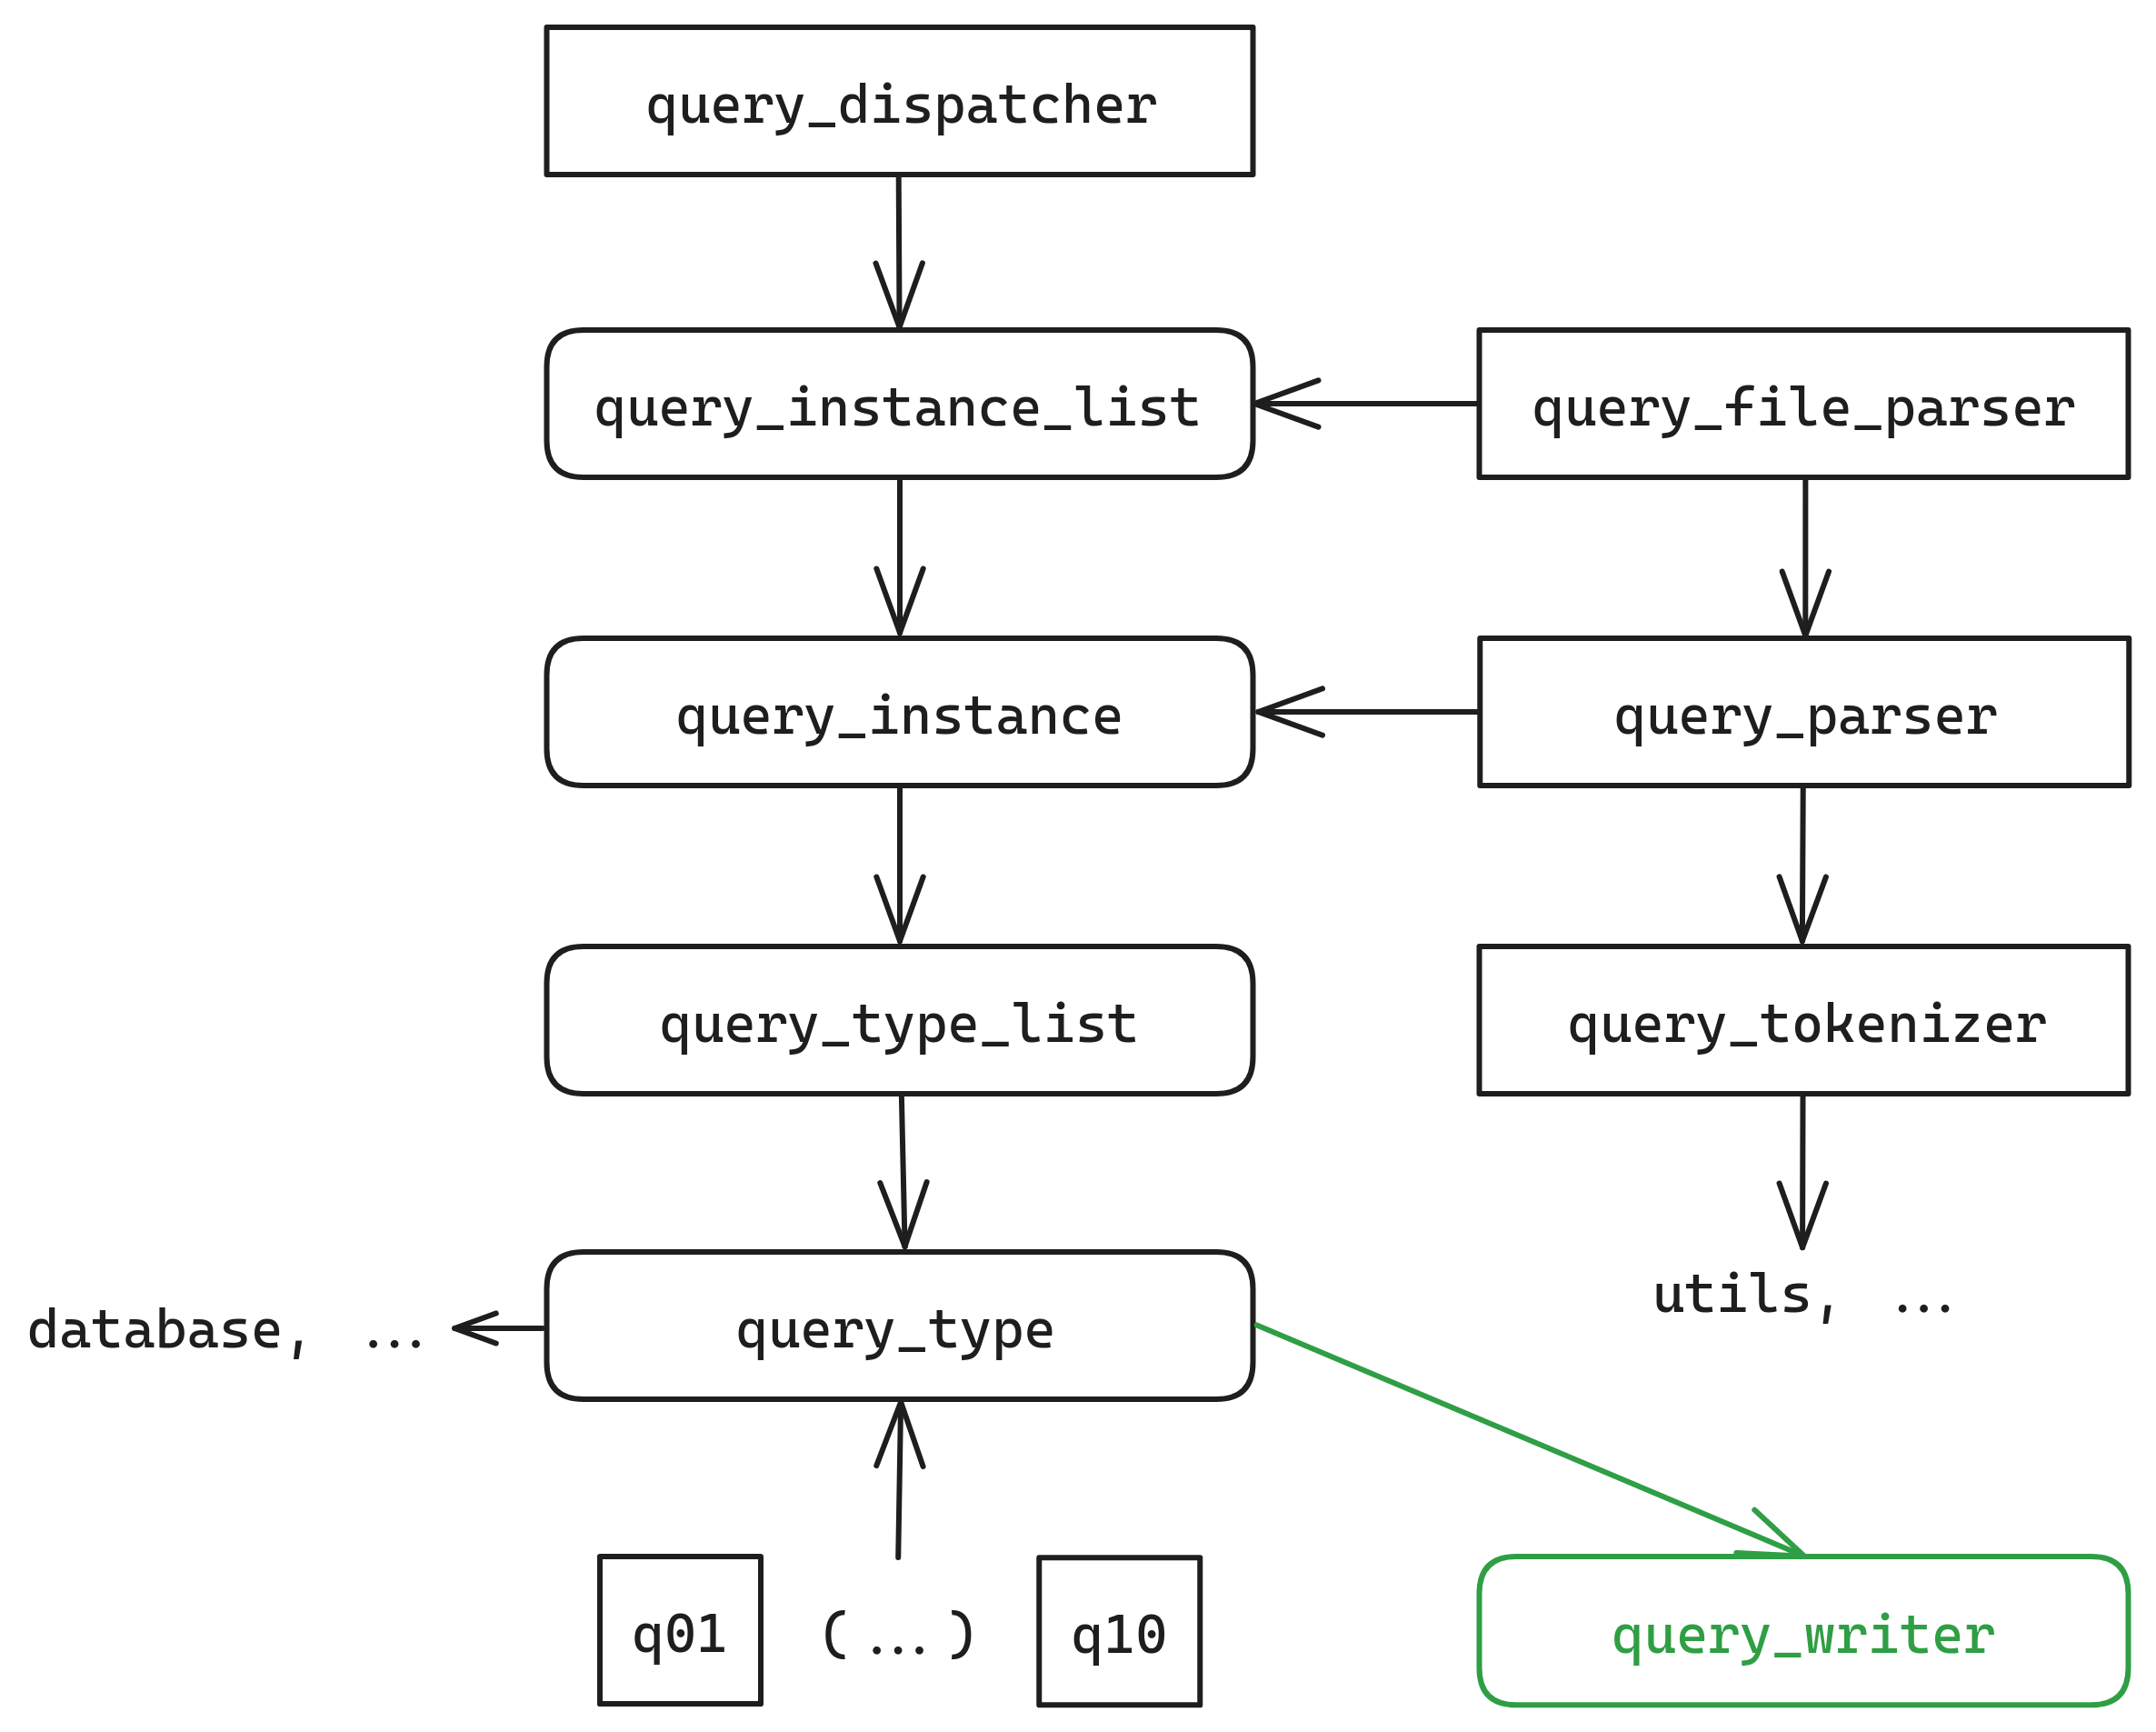
\includegraphics[scale=0.17]{res-fase2/queries.png}
    \caption{Diagrama de dependências do subsistema de \emph{queries}}
    \label{fig:queries}
\end{figure}

Como todas as \emph{queries} apresentam a mesma formatação de \emph{output}, adicionámos a estrutura
\texttt{query\_writer}, que formata o \emph{output} de uma \emph{query} automaticamente, e escreve-o
para um ficheiro (modo \emph{batch}) ou para um conjunto de linhas em memória (modo interativo).
Segue-se a descrição do funcionamento das \emph{queries} novas e das que sofreram mudanças
significativas:

\begin{itemize}
    \item \textbf{Q05} - Listagem dos voos com origem num dado aeroporto entre duas datas. Com uma
                         única iteração pelos voos para todas as \emph{queries} deste tipo,
                         verifica-se se cada voo cumpre as condições para ser parte da resposta
                         de uma \emph{query}. Em caso afirmativo, adiciona-se esse voo a um
                         \emph{array}, associado à \emph{query} através de uma tabela de
                         \emph{hash}. Após cada \emph{array} ser ordenado, a execução de cada
                         \emph{query} consiste simplesmente na exibição dos seus conteúdos.

    \item \textbf{Q07} - Listagem dos aeroportos com maior mediana de atrasos. Inicia-se com uma
                         tabela de \emph{hash} que associa aeroportos a \emph{arrays} de números
                         correspondentes a atrasos. Com uma única iteração pelos voos para todas
                         as \emph{queries} deste tipo, preenche-se o \emph{array} de cada aeroporto
                         com os atrasos dos seus voos. No fim, ordena-se cada \emph{array} e gera-se
                         uma tabela de \emph{hash} entre aeroportos e atrasos. A execução de uma
                         \emph{query} individual consiste na consulta dos maiores elementos desta
                         tabela.

    \item \textbf{Q08} - Cálculo da receita de um hotel entre duas datas. Com uma única iteração
                         pelas reservas para todas as \emph{queries} deste tipo, gera-se uma tabela
                         de \emph{hash} que associa pares hotéis + datas às suas receitas. A cada
                         reserva, calcula-se o número de noites simultaneamente dormidas e no
                         intervalo da \emph{query}, para se calcular a receita resultante dessa
                         reserva. A execução de cada \emph{query} consiste simplesmente na consulta
                         da tabela gerada.

    \item \textbf{Q09} - Listagem de todos os utilizadores cujo nome comece com um dado prefixo. A
                         nova implementação desta \emph{query} é muito semelhante à da \textbf{Q5},
                         mas com uma iteração pelos utilizadores em vez dos voos. Esta solução é
                         significativamente mais veloz que a anterior, que iterava pelos
                         utilizadores uma vez para cada \emph{query}. Considerámos a possibilidade
                         de geração da um índice usando \emph{tries}, mas o seu elevado uso de
                         memória não é compensador, dado que muito pouco do tempo total do programa
                         é passado na execução desta \emph{query}.

    \item \textbf{Q10} - {\color{red}Ainda tenho de implementar isto}
\end{itemize}

\subsection{Modo interativo}
\label{sec:interactive-mode}

\begin{figure}[ht]
    \centering
    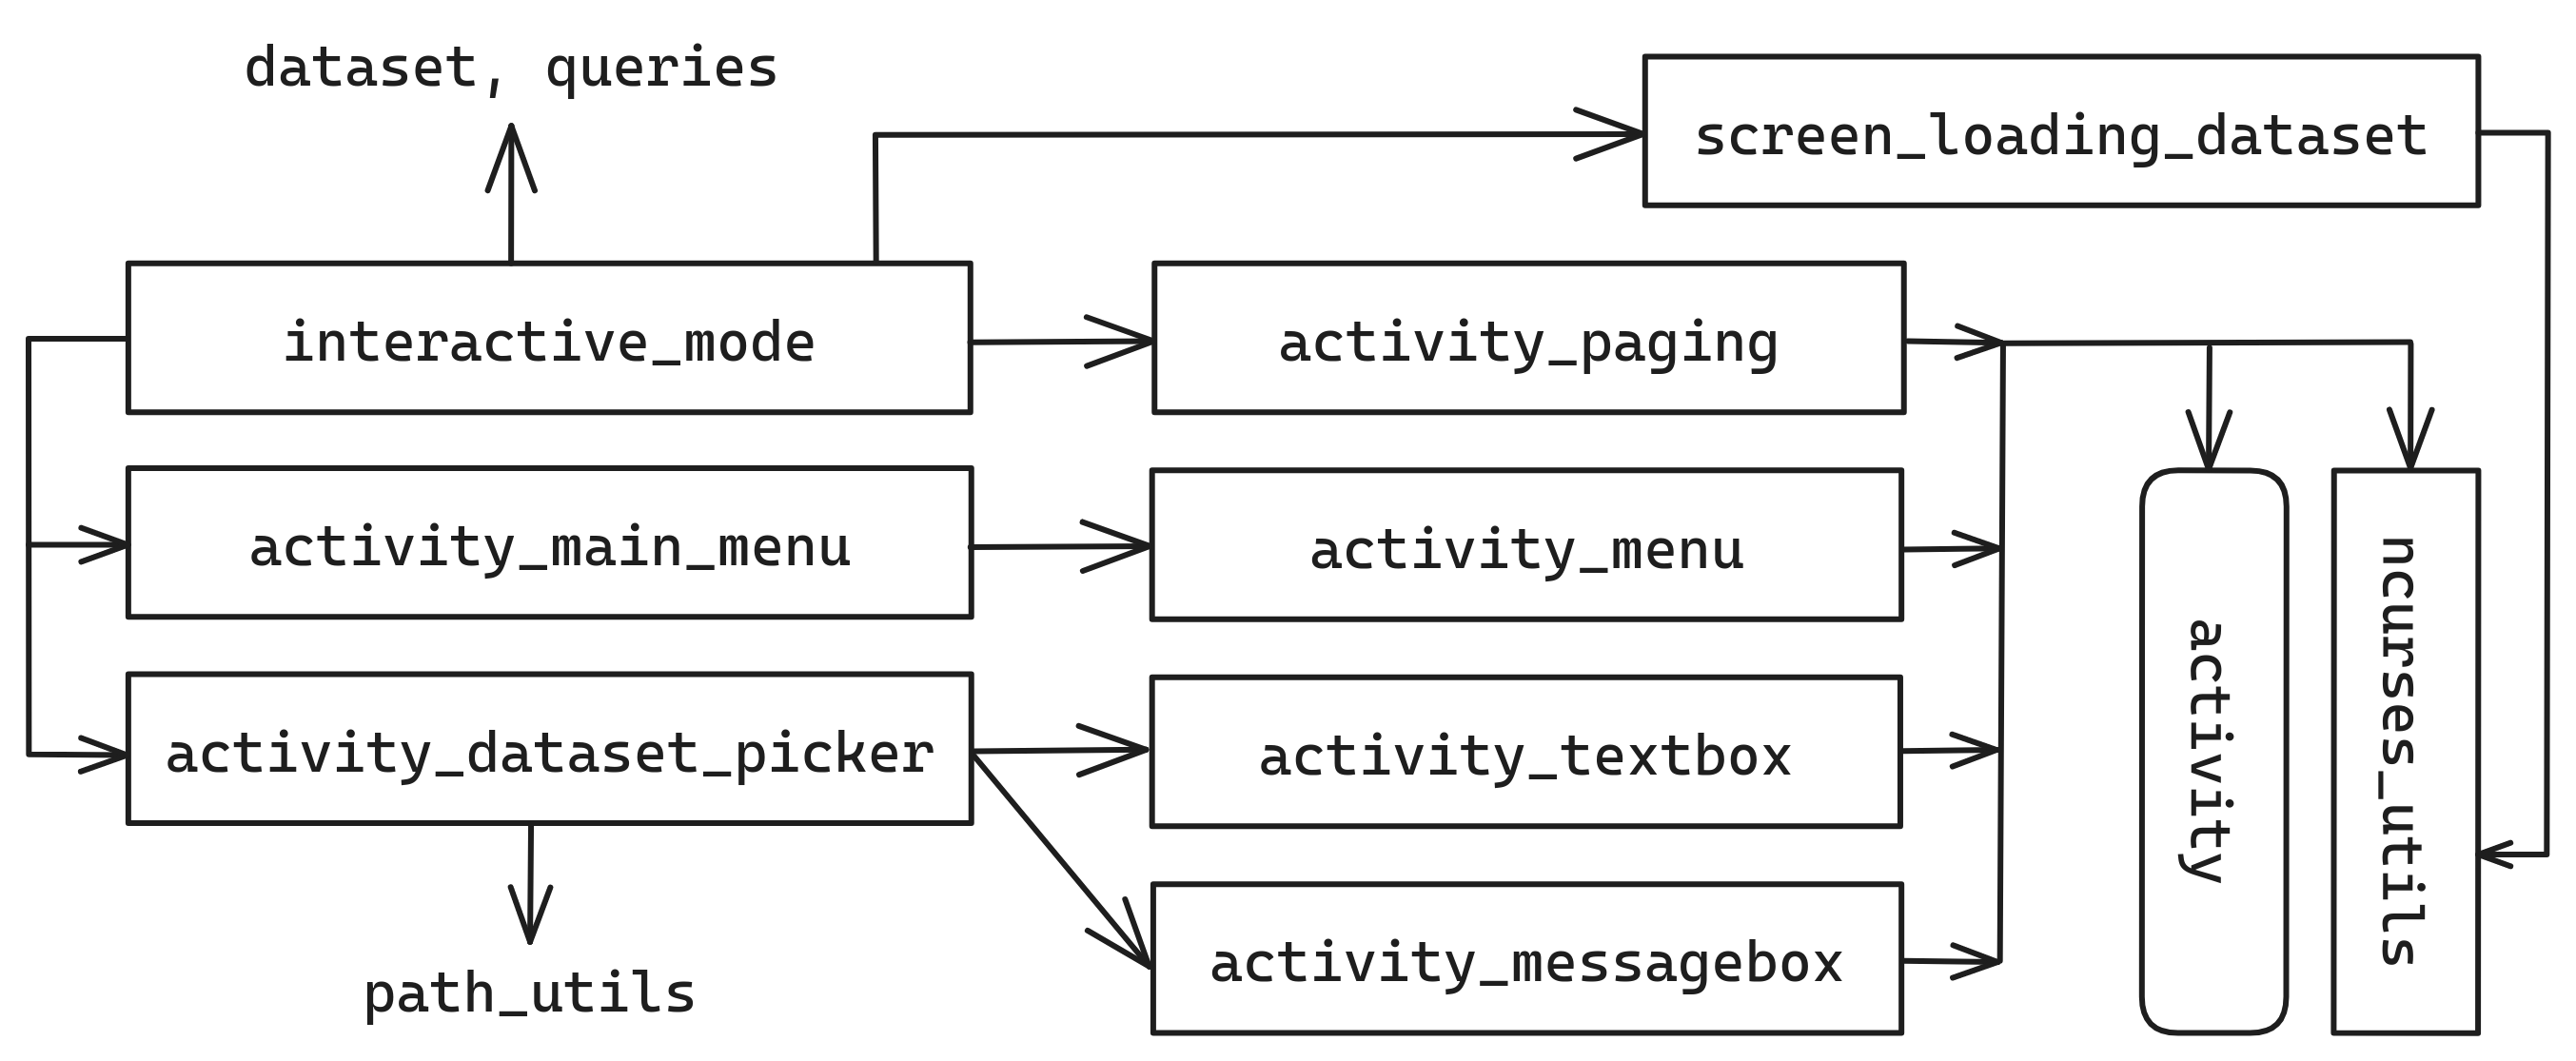
\includegraphics[scale=0.17]{res-fase2/interactive.png}
    \caption{Diagrama de dependências do modo interativo}
    \label{fig:interactive}
\end{figure}

O modo interativo revolve à volta do conceito de atividade (\texttt{activity}), que gere o
\emph{loop} de eventos de uma interface \texttt{curses}, chamando os \emph{callbacks} com os quais
é definida para responder a esses eventos. Imagens de cada uma destas atividades podem ser
encontradas em \nameref{sec:interactive-screenshots}. \texttt{screen\_loading\_dataset} não responde
a eventos, mas desenha no ecrã que a aplicação se encontra a ler um \emph{dataset}. O módulo
\texttt{interactive\_mode} é responsável por controlar a troca entre atividades, formando a
aplicação final.

Fizemos questão de que o modo interativo fosse fácil de utilizar: incluímos instruções em todas as
interfaces, e desenvolvemos um navegador de ficheiros para o utilizador não ter de digitar um
caminho de ficheiro. Ademais, temos excelente suporte para Unicode, com medição textual correta para
o \emph{layout} das interfaces (alguns caracteres podem ser mais longos que outros, situação
com a qual o nosso programa lida corretamente).

\subsection{Subsistema de testes}
\label{sec:testing-subsystem}

\begin{figure}[ht]
    \centering
    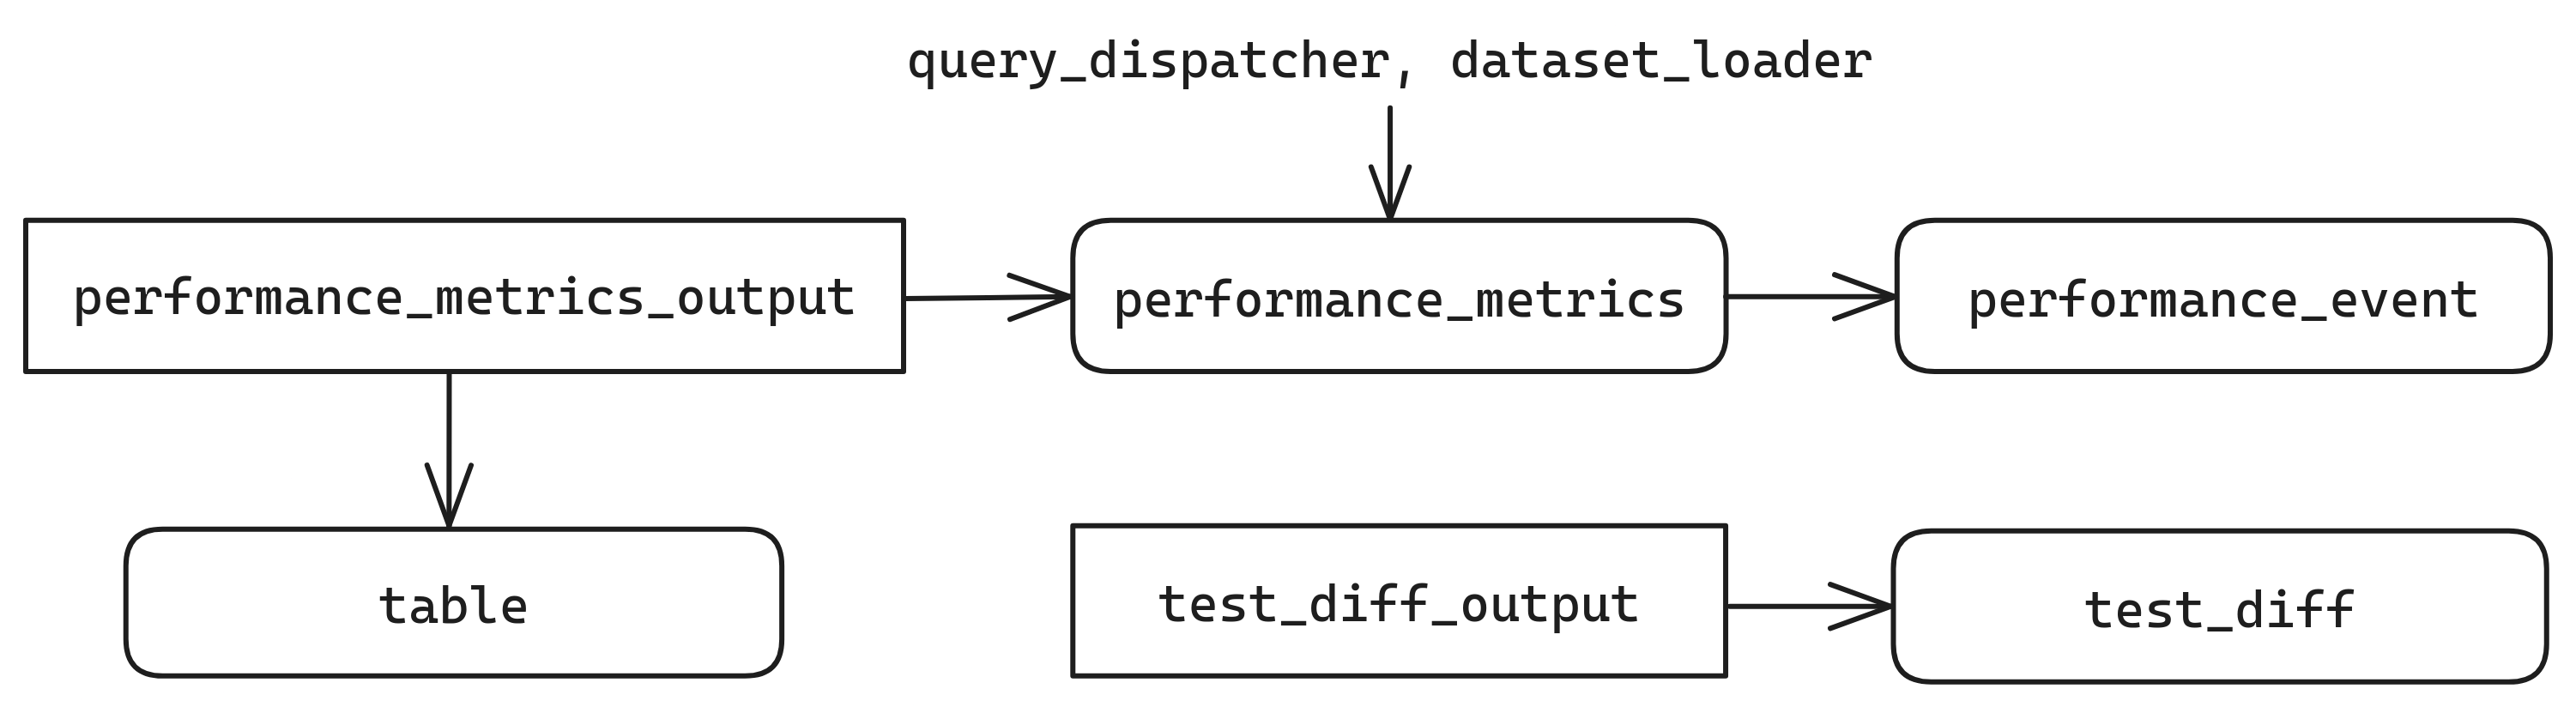
\includegraphics[scale=0.15]{res-fase2/testing.png}
    \caption{Diagrama de dependências do subsistema de testes}
    \label{fig:testing}
\end{figure}

Os testes de desempenho baseiam-se num \texttt{performance\_event}, uma medição do tempo e da
diferença do uso de memória entre dois instantes. \texttt{performance\_metrics} são um conjunto de
eventos de desempenho, que são produzidos ao longo do decorrer da aplicação, e mostrados ao
utilizador no final da sua execução pelo módulo \texttt{performance\_metrics\_output}. São
apresentadas várias tabelas (\texttt{table}), relativas ao uso de recursos computacionais na leitura
de cada parte do \emph{dataset} e na execução de cada \emph{query} (tempo individual, estatístico e
amortizado).

Os testes funcionais são implementados por \texttt{test\_diff}, que calcula as diferenças entre
duas diretorias (ficheiros em falta, em excesso, e diferenças entre ficheiros), que são depois
apresentadas ao utilizador por \texttt{test\_diff\_output}.

\section{Modularidade e encapsulamento}
\label{sec:modularity-and-encapsulation}

\subsection{Modularidade}
\label{sec:modularity}

No relatório da primeira fase, afirmámos estar, de um modo geral, satisfeitos com o nível de
modularidade conseguido. No entanto, tínhamos noção de que havia alguns detalhes a corrigir,
nomeadamente, separar o I/O das \emph{queries} e do \emph{dataset}, e criar módulos para os
identificadores de hotéis, voos e reservas, que continham código anteriormente replicado por toda a
\emph{codebase}. Não só corrigimos estes problemas, como planeámos as novas partes da aplicação
tendo em conta as anteriores falhas na estrutura do programa.

\subsection{Encapsulamento}
\label{sec:encapsulation}

\subsubsection{\emph{The great refactoring}}
\label{sec:the-great-refactoring}

Apesar de, na primeira fase deste trabalho, termos definido \emph{getters} e \emph{setters} para as
estruturas de dados, estávamos cientes da ausência de encapsulamento, pois vários \emph{getters}
devolviam apontadores mutáveis para dados no interior das estruturas. Sabíamos que seria ao
encapsulamento que se dedicaria a maior parte do esforço da 2.ª fase, o que se provou verdade. Como
apenas líamos informação dos apontadores mencionados, sem nunca escrever, tornar esses apontadores
constantes provou-se a melhor solução para o encapsulamento.

No entanto, neste processo de aplicar a \emph{keyword const} aos argumentos dos métodos e aos seus
valores devolvidos, apercebemo-nos da importância de uma interface modular bem pensada que
dispense mudanças. A cada \emph{const} adicionado, vários módulos deixavam de compilar por erros de
tipos, deixando-nos num processo de horas de correções sem conseguir compilar o projeto, com medo de
que alguma mudança que fizéssemos causasse algum erro que não saberíamos depurar. Felizmente, poucos
foram estes erros, e todos fomos capazes de resolver com facilidade.

No modo interativo e no subsistema de testes, como pensámos nas interfaces dos módulos com
encapsulamento em mente, não precisámos de gastar tempo na sua correção. Ademais, adicionámos
métodos de cópia profunda (semelhantes aos \emph{copy constructors} de C++) a todas as estruturas
de dados da aplicação\footnote{Com exceção de alocadores (\emph{pools}) e estruturas que contêm
\emph{handles} de ficheiros (não é possível copiar um \texttt{FILE *}).} que, apesar de não
utilizarmos, são cruciais para a extensibilidade da aplicação, caso algo que se pretenda fazer
exija a criação de cópias de certas estruturas.

\subsubsection{Conciliação com alocadores}
\label{sec:allocator-conciliation}

As únicas estruturas de dados que expõem memória do seu interior são os alocadores \texttt{pool} e
\texttt{string\_pool}. Não encaramos isto como um problema no encapsulamento, pois é algo que
qualquer alocador tem de fazer (por exemplo, o método \texttt{malloc} expõe memória da arena com
que é implementado).

No entanto, previamente, durante uma adição à base de dados, os campos das novas entidades eram
alocados pelos \emph{managers} nas \emph{pools}, e não pelas entidades em si, tratando-se de um
verdadeiro problema no encapsulamento. Resolvemo-lo usando uma estratégia semelhante à utilizada na
linguagem Zig, que aplicámos apenas às entidades: se um método precisa de alocar memória na
\emph{heap}, então leva um alocador como argumento, que usa para as alocações necessárias:

\begin{center}
    \texttt{fn validate(allocator: Allocator, s: []const u8) Allocator.Error!bool}
\end{center}

Este método de Zig valida texto JSON, levando também como argumento um alocador e podendo devolver
ou um booleano ou um erro de alocação. Na nossa aplicação C, é dada a possibilidade de se usar uma
\emph{pool}, ou de se passar o valor \texttt{NULL} a esse argumento para o uso de \texttt{malloc}:

\begin{center}
    \begin{tabular}{rl}
		\texttt{user\_t *user\_clone(}&\hspace{-3mm}\texttt{pool\_t *allocator,} \\
        &\hspace{-3mm}\texttt{string\_pool\_t *string\_allocator,} \\
        &\hspace{-3mm}\texttt{const user\_t *user);}
    \end{tabular}
\end{center}

\subsubsection{Conciliação com a \texttt{glib}}
\label{sec:glib-conciliation}

{\color{red} I still need to think how to handle this}

\section{Desempenho}
\label{sec:performance}

\subsection{Melhorias}
\label{sec:performance-improvements}

Dado que o nosso grupo se preocupou com o desempenho da aplicação já desde a primeira fase do
projeto, quando os \emph{datasets} de maior dimensão foram adicionados à plataforma de testes,
o nosso programa correu em tempo e memória muito inferiores aos limites de recursos máximos. Mesmo
assim, procurámos continuar a aumentar o desempenho da nossa aplicação.

Para reduzir ainda mais o uso de memória, introduzimos a \texttt{string\_pool\_no\_duplicates}, que
evita armazenar \emph{strings} repetidas. Ademais, reordenamos os campos nas estruturas de dados das
entidades, de modo a reduzir o \emph{padding} e o número de \emph{bytes} ocupados por cada uma.

A maioria do tempo de tempo de execução é gasto no \emph{parsing} do \emph{dataset}, pelo que
procurámos alcançar micro-otimizações nos métodos mais chamados, determinados com recurso ao
\texttt{callgrind}. A única melhoria significativa que obtivemos resultou da substituição do
\texttt{strsep} por um novo método que considera apenas um delimitador.

Ademais, como a execução das \emph{queries} já era muito veloz devido à localidade de memória
(tanto o custo amortizado como o do modo interativo), o nosso foco foi o de simplificar o código, e
não o de o otimizar com melhores estruturas de dados. Tal provou-se vantajoso, pois várias vezes as
estruturas simples se provaram mais rápidas do que outras mais complexas, uma lembrança de que a
complexidade algorítmica é assintótica. Foi importante garantir que os catálogos usavam as
melhores estruturas para responder às relações pedidas pelas \emph{queries}, mas tal não se provou
tão relevante para dados auxiliares usados durante a execução das mesmas.

\subsection{\emph{Benchmarking}}
\label{sec:benchmarking}

% TODO - benchmarking

\subsection{Possíveis melhorias}
\label{sec:possible-performance-improvements}

{\color{red} Falar um pouco de multithreading só para chatear}

\pagebreak
\section{Anexos}
\label{sec:annexes}

\subsection{Diagrama de dependências completo}
\label{sec:complete-diagram}

% TODO - full dependency diagram

\subsection{\emph{Screenshots} do modo interativo}
\label{sec:interactive-screenshots}

\begin{figure}[ht]
    \centering
    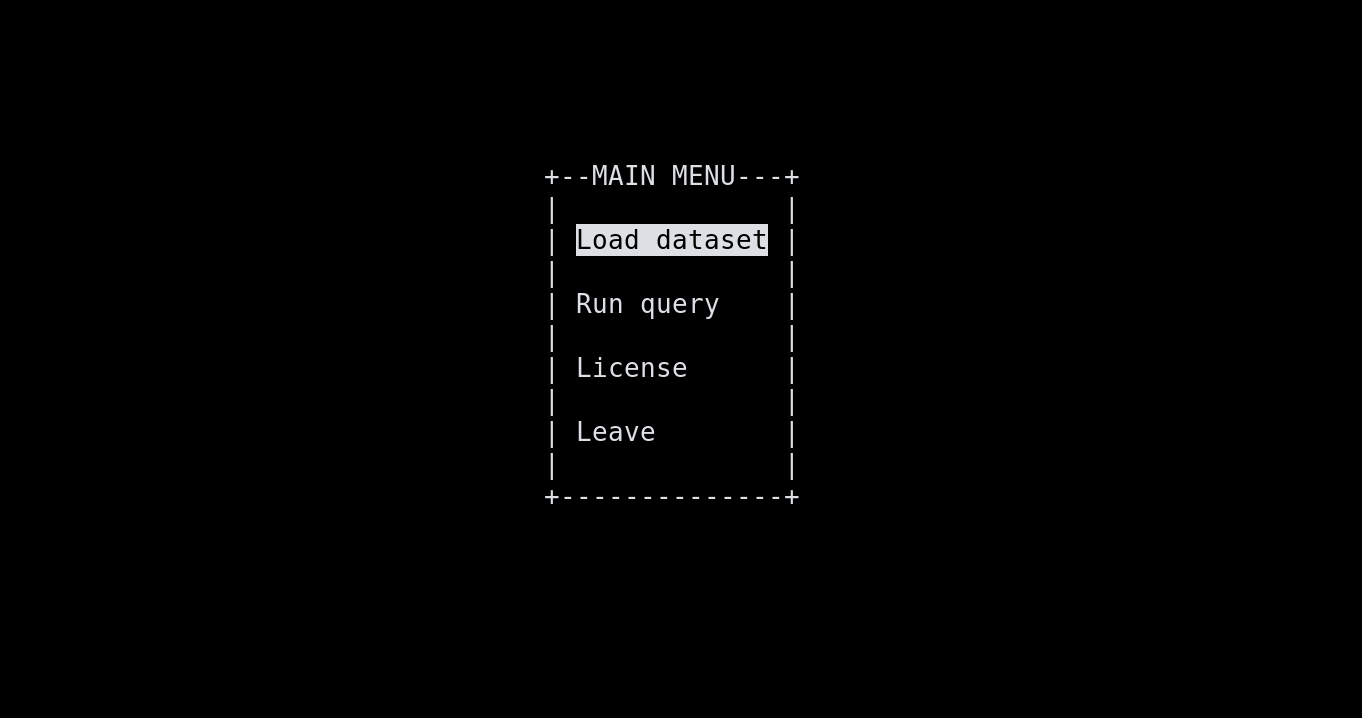
\includegraphics[scale=0.25]{res-fase2/interactive_screenshots/main_menu.png}
    \caption{Menu (\texttt{activity\_menu}), em particular, o menu principal
             (\texttt{activity\_main\_menu})}
    \label{fig:main_menu}
\end{figure}

\begin{figure}[ht]
    \centering
    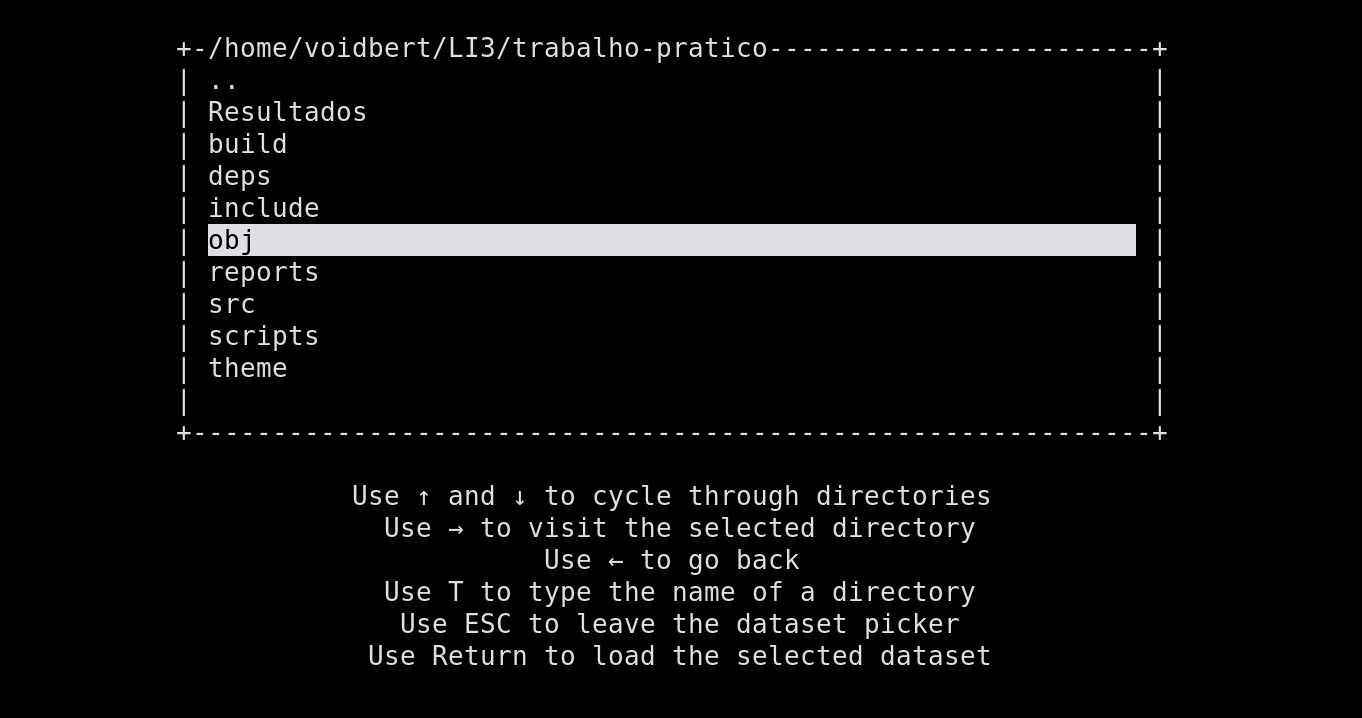
\includegraphics[scale=0.25]{res-fase2/interactive_screenshots/dataset_picker.png}
    \caption{Navegador de ficheiros para a escolha de um \emph{dataset}
             (\texttt{activity\_dataset\_picker})}
    \label{fig:dataset_picker}
\end{figure}

\begin{figure}[ht]
    \centering
    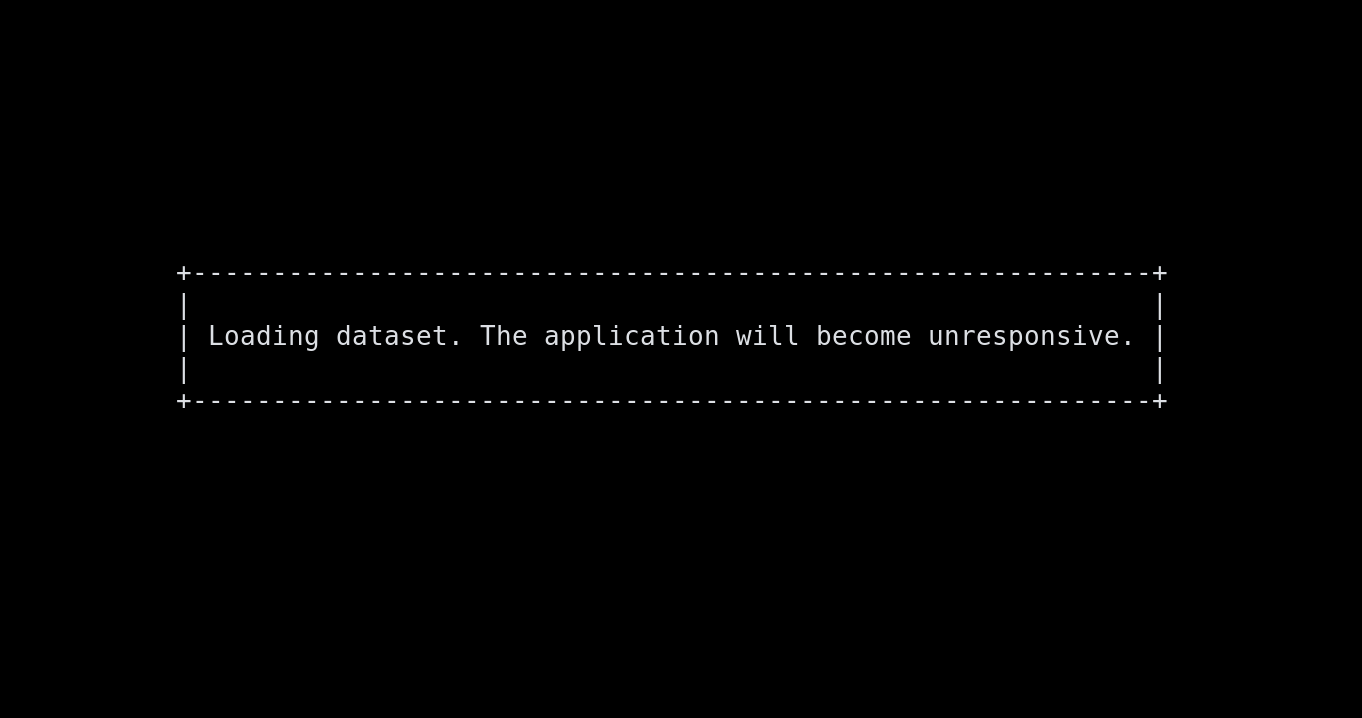
\includegraphics[scale=0.25]{res-fase2/interactive_screenshots/loading_dataset.png}
    \caption{Ecrã durante a leitura de um \emph{dataset} (\texttt{screen\_loading\_dataset})}
    \label{fig:loading_dataset}
\end{figure}

\begin{figure}[ht]
    \centering
    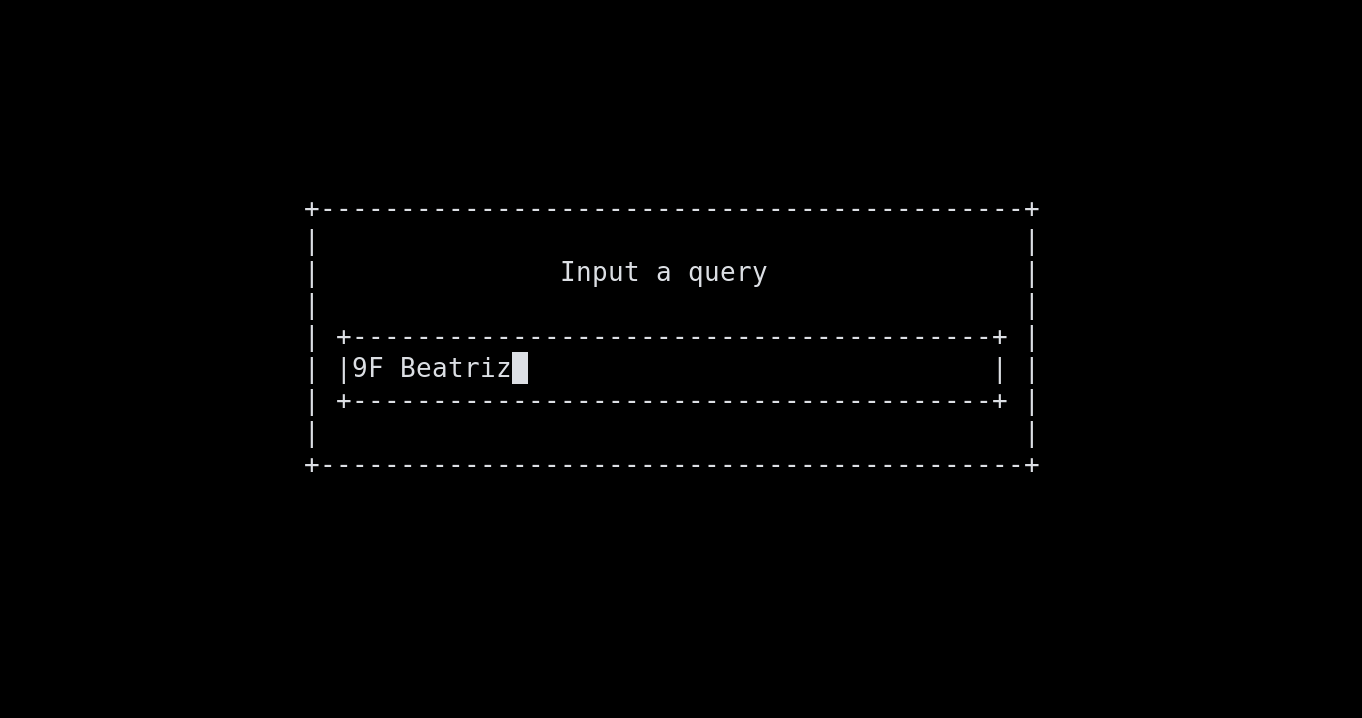
\includegraphics[scale=0.25]{res-fase2/interactive_screenshots/textbox.png}
    \caption{Caixa de texto para a entrada de uma \emph{query} (\texttt{activity\_textbox})}
    \label{fig:textbox}
\end{figure}

\begin{figure}[ht]
    \centering
    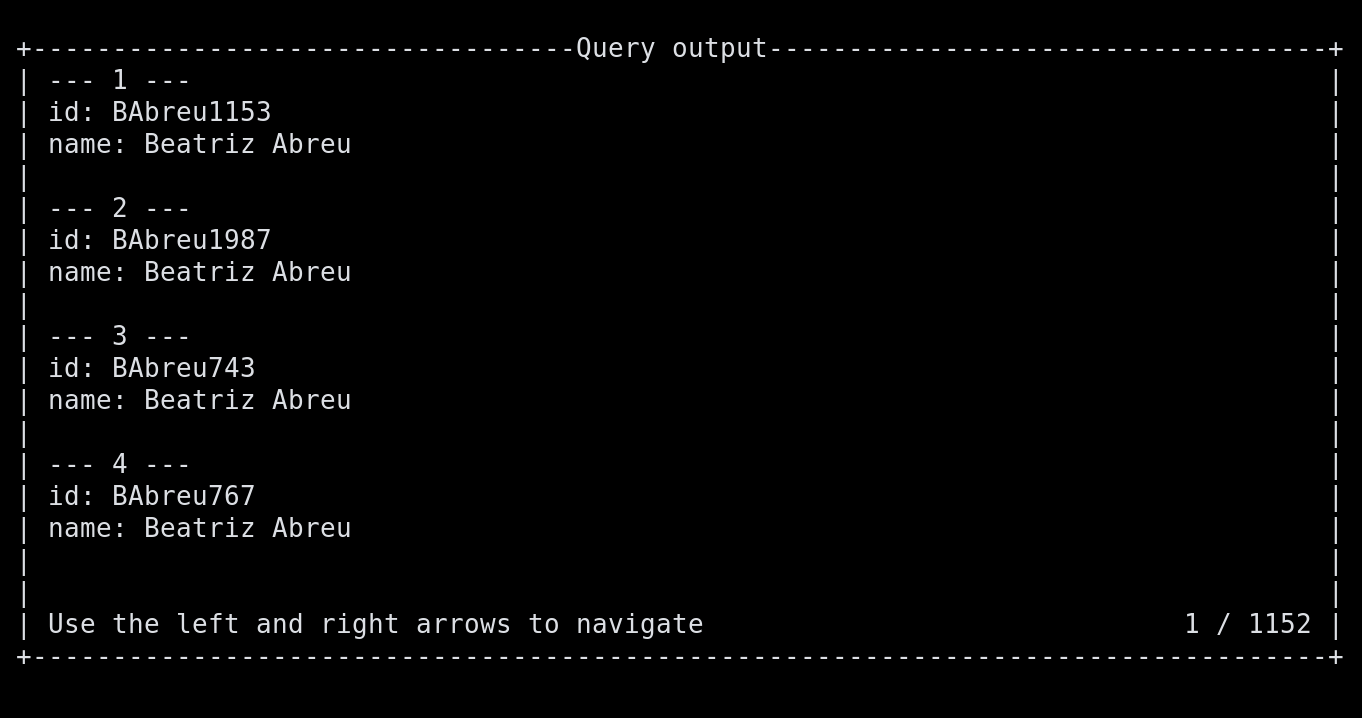
\includegraphics[scale=0.25]{res-fase2/interactive_screenshots/paging.png}
    \caption{Output paginado de uma \emph{query} (\texttt{activity\_paging})}
    \label{fig:paging}
\end{figure}

\begin{figure}[ht]
    \centering
    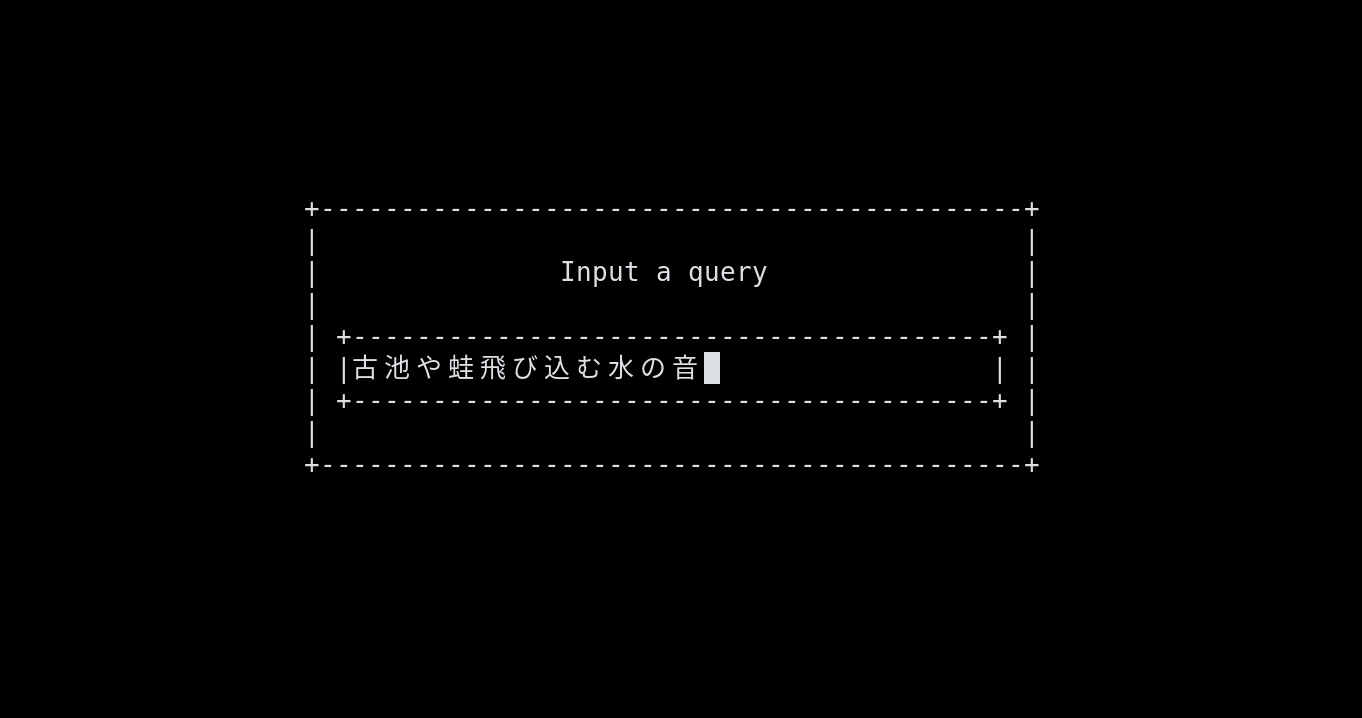
\includegraphics[scale=0.25]{res-fase2/interactive_screenshots/japanese.png}
    \caption{Suporte para caracteres de largura dupla numa \texttt{activity\_textbox}.
             O \emph{scrolling} mantém-se funcional.}
    \label{fig:japanese}
\end{figure}

\begin{figure}[ht]
    \centering
    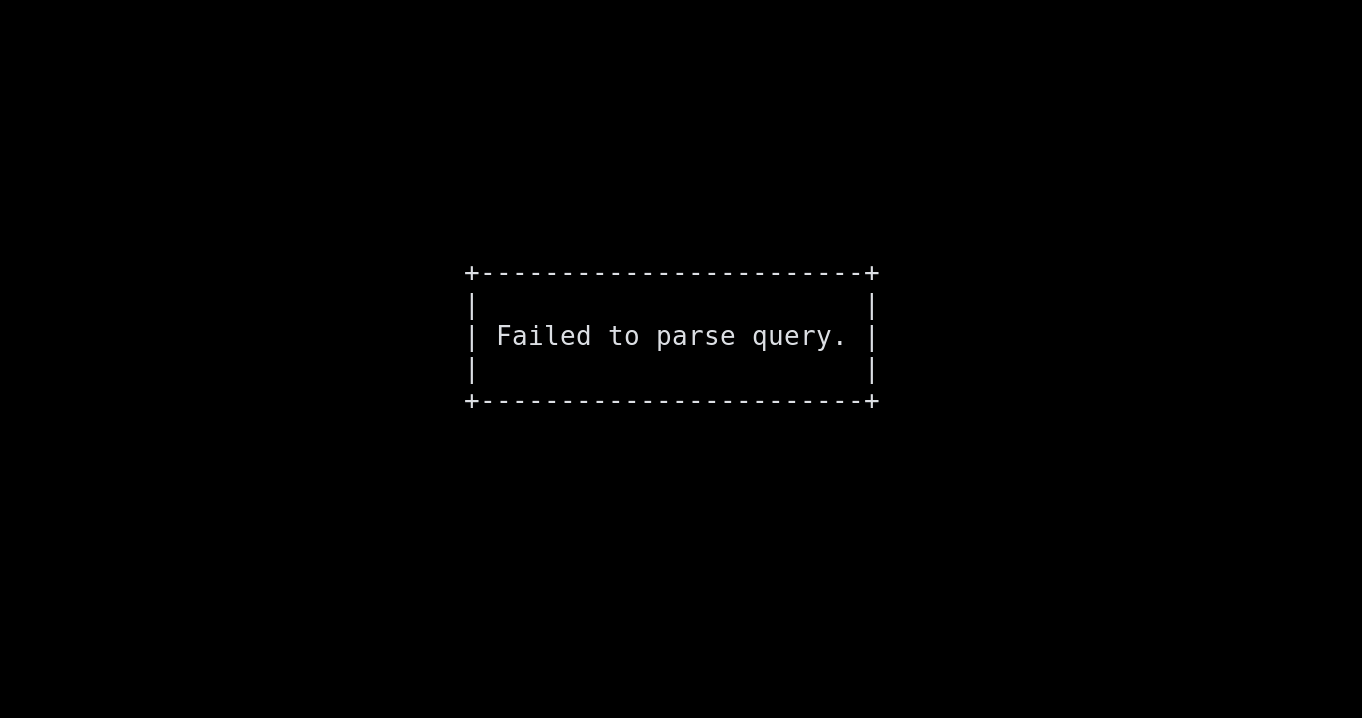
\includegraphics[scale=0.25]{res-fase2/interactive_screenshots/messagebox.png}
    \caption{Aviso de erro numa \texttt{activity\_messagebox}}
    \label{fig:messagebox}
\end{figure}

\end{document}
